\documentclass[../../thesis.tex]{subfiles}
\graphicspath{{\subfix{diagrams/}}}

% \begin{document}
To analyze the systems performance, there are two different metrics to look at, the gas consumption of an aggregation batch and the execution time needed for the zkSNARK proof generation. We will start of with the gas consumption, and then move on to the zkSNARK metrics.

\subsection{Gas Usage}
This system has four different operations that use gas to be executed. 

\paragraph{Trade Aggragation}
To break down the costs of a trade aggregation batch, we must first differentiate between fixed and variable gas cost that need to be paid per batch. For one, the gas for the net trade, executed on Uniswap, must be paid. This amount varyies, depending on the direction of the net trade, ~142k when trading from eth and ~167k gas when trading from a token. Since the direction of the net trade can't be predicted, we will work with the higher value for the break even point as seen in F. \ref{fig:cost_trade}. 
 
Another fixed cost to consider is the costs of verifying the zkSNARK proof, along with handling the refund payment of the aggregator and some other checks in the zkSwap smart-contract. Executing these costs ~342k gas per aggregation batch. The combined fixed amount of gas per aggregation batch is ~484k/~509k gas, depending on the net trade direction. For each trade in a batch, we must pay 6619 gas, which is used for recreating the data hash, as well as emitting the BalanceUpdate event. When using these numbers, we get the following cost per trade, depending on the batch size. This chart can also be found trading from Ether in the appendix, where the cost per trade is slightly lower. As these values converge very quickly, the chart is omited here. The theoretical maximum batch size is 1811, which is where Ethereums block gas limit is reached. 

\begin{figure}[h]
    \centerline{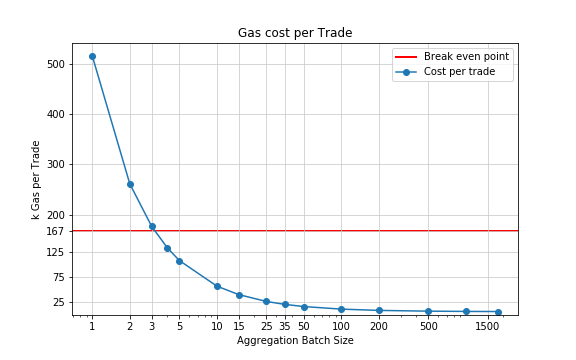
\includegraphics[totalheight=6cm]{diagrams/trade_cost.png}}
    \caption{Gas cost per trade and breakeven point}
    \label{fig:cost_trade}
\end{figure}


\subsection{zkSNARK Circuit Metrics}
Another aspect to consider is the performance of the zkSNARK circuits. The benchmarks for the zkSNARK circuits where performed on a Google Cloud Plattform C2 instance, with 60 vCores (3.1GHz base and 3.8GHz turbo) and 240Gb of memory. This instance was chosen because of the large amount of memory and the fast clock speed. The number of cores doesn’t impact the benchmarking results, as the zkSNARK proof aggregation steps can’t be parallelised at the time of writing.

\subsubsection{Execution Time}
The first obvious metric to consider is execution times of the different steps required to generate a proof. 

\paragraph{Compilation and Setup}
Before we can generate any zkSNARK proofs, we have to compile our circuits and run the setup. These two steps only need to be run once per circuit, so they're not significant for the viablilty of this system. However I have the numbers, and it would feel incomplete to not present them. These are the results, for the trade and deposit/withdraw circuit.

\begin{figure}[h]%
    \centering
    \subfloat[]{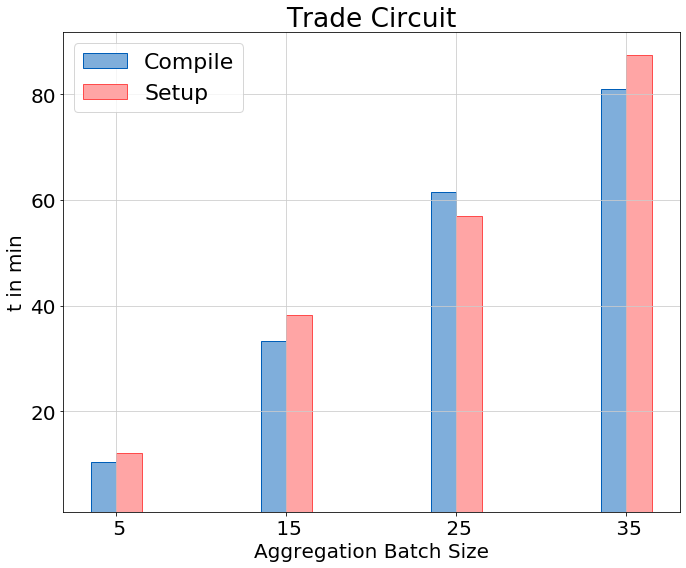
\includegraphics[width=5.9225cm]{diagrams/results_final_trade-compile-setup-time.png} }%
    \qquad
    \subfloat[]{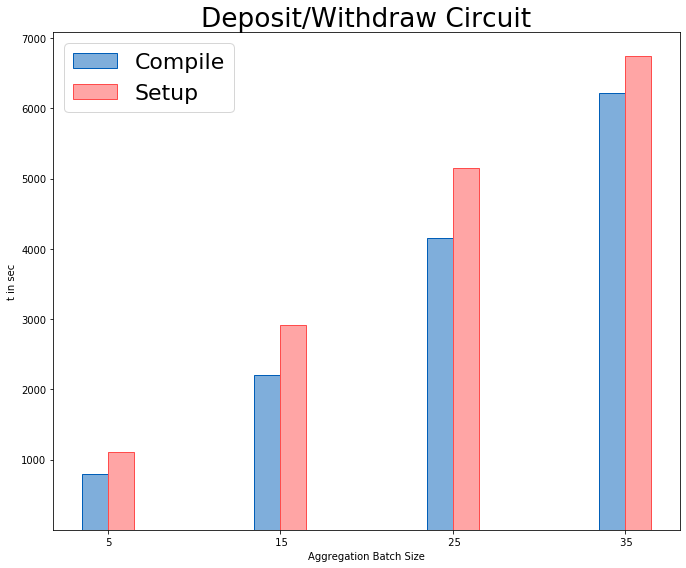
\includegraphics[width=5.9225cm]{diagrams/results_final_dep-compile-setup-time.png} }%
    \caption{Compilation and setup execution times}%
    \label{fig:comp_setup_time}%
\end{figure}

\paragraph{Witness Computations and Proof Generation}
For each aggregation batch we need to first run the witness computation, after which the proof generation can be run. These two steps need to be run for every aggregation batch, so the performance is a indicator for the viability of this system. It decides how long the aggregation of a batch takes, which impacts the pratical application of this system. 

\begin{figure}[h]%
    \centering
    \subfloat[]{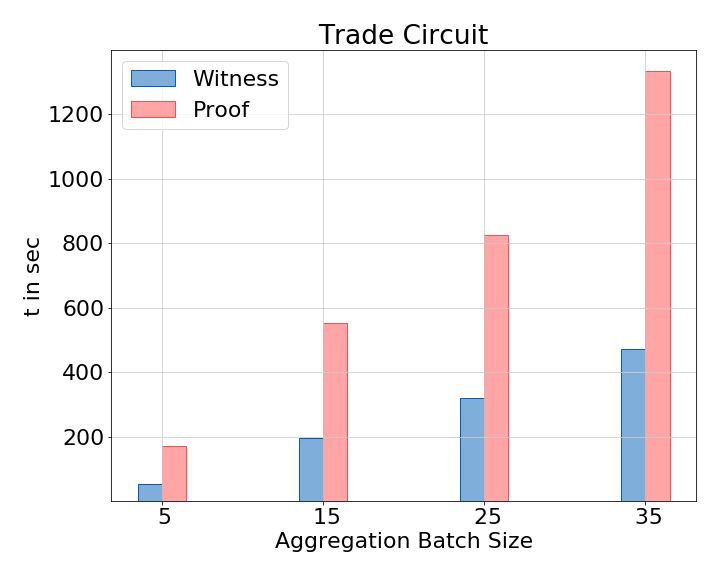
\includegraphics[width=5.9225cm]{diagrams/results_final_trade-witness-proof-time.png} }%
    \qquad
    \subfloat[]{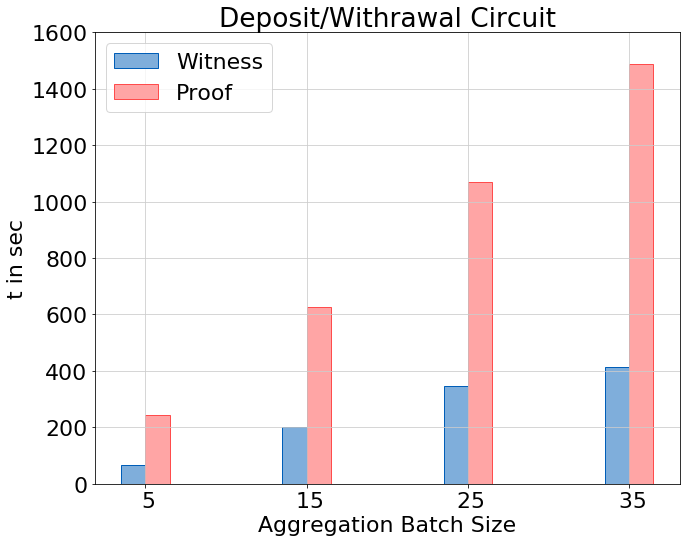
\includegraphics[width=5.9225cm]{diagrams/results_final_dep-witness-proof-time.png} }%
    \caption{Witness computation and proof generation}%
    \label{fig:witness_proof_time}%
\end{figure}

\subsubsection{Memory Usage}
Only looking at the execution times gives us an idea how many operation can be batched. It tells us nothing about the hardware requirements needed for working with circuits of this size. One thing to look at, is the memory used in the different steps. In general, the memory consumption of these processes is high, which is why a server instance with such a large amount of memory was chosen. 

\paragraph{Compilation and Setup}
When measuring the compilation memory consumption, we get a confusing picture. The results don't really make sense, as smaller circuits sometimes require more memory as smaller ones. However, I repeated this measurement on different machines and operating systems, always receiving inconclusive results, similar to these. I watched the compilation on the server with htop, and observed the same amount of memory that the memory usage script was detecting. The script uses the command line tool `ps' to take these measurements, which measures reserved memory by a process. Alternativly, a profiler could be used to measure the actual memory usage. This would impact the performance of the application severly though. As these steps only have to executed once, they are not a meaningful metric. 

\begin{figure}[h]%
    \centering
    \subfloat[]{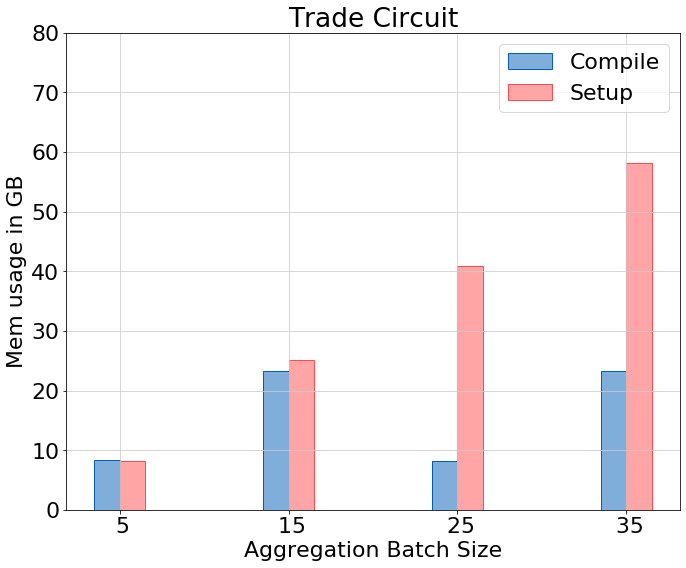
\includegraphics[width=5.9225cm]{diagrams/results_final_trade-compile-setup-mem.png} }%
    \qquad
    \subfloat[]{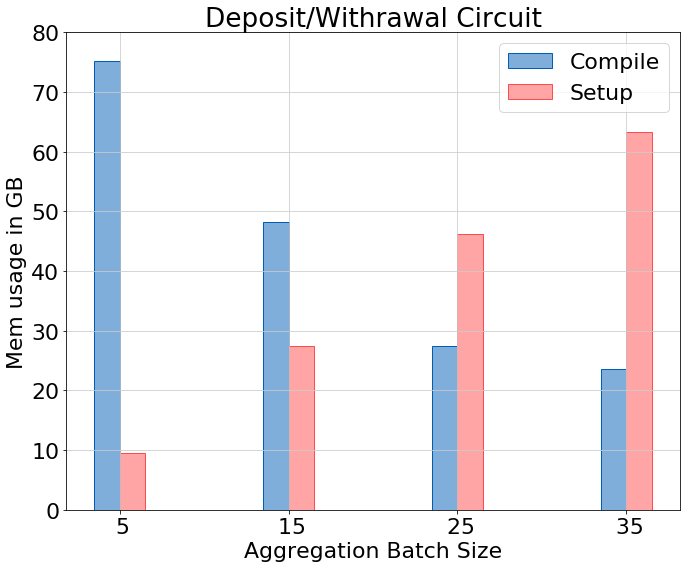
\includegraphics[width=5.9225cm]{diagrams/results_final_dep-compile-setup-mem.png} }%
    \caption{Compilation and setup memory consumption}%
    \label{fig:comp_setup_mem}%
\end{figure}

\paragraph{Witness Computation and Proof Generation}
The memory required for running the witness computation and proof generation is an important metric and dictates the hardware needed for the aggregation process. As we can see, running this requires a large amount of memory. 

\begin{figure}[h]%
    \centering
    \subfloat[]{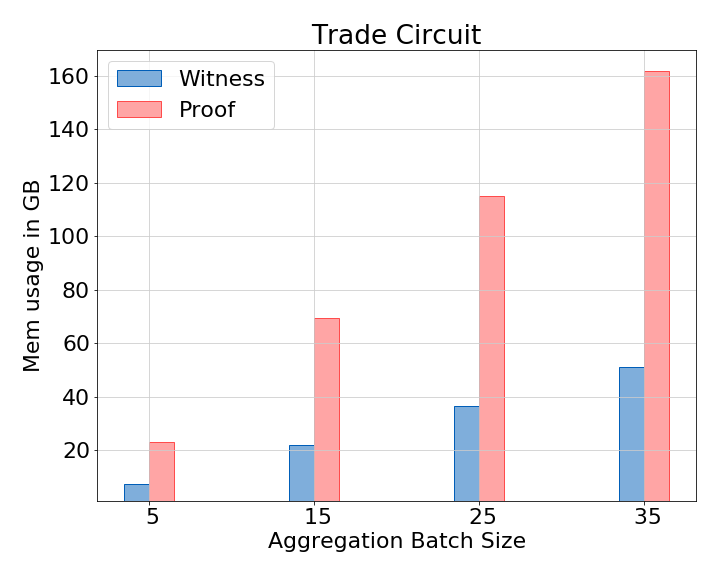
\includegraphics[width=5.9225cm]{diagrams/results_final_trade-witness-proof-mem.png} }%
    \qquad
    \subfloat[]{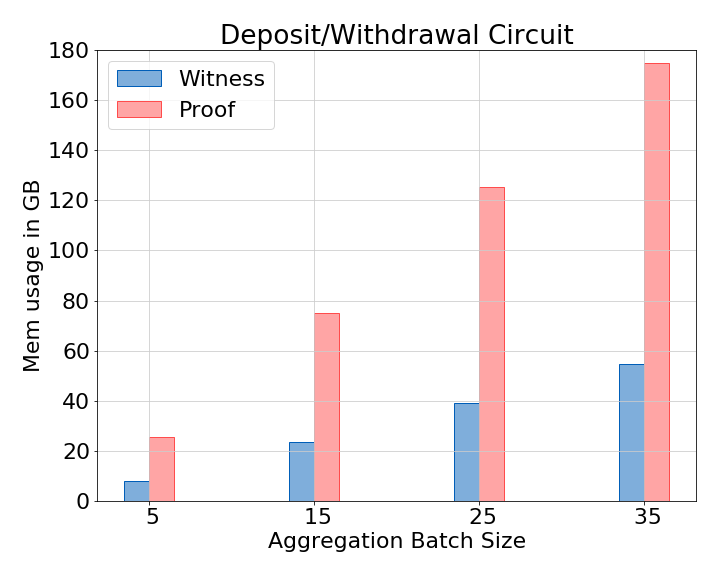
\includegraphics[width=5.9225cm]{diagrams/results_final_dep-witness-proof-mem.png} }%
    \caption{Witness computation and proof generation memory consumption}%
    \label{fig:witness_proof_mem}%
\end{figure}

\subsubsection{Constraints}
Looking at the results, we see that the execution times increase linearly with the batch size. The same pretty much goes for the memory consumption of our circuits. As a general rule, the complexity of a zkSNARK circuit is defined by amount of constraint the circuit is made of. Each additional element in the batch adds a certain number of constraints to the circuit.  Looking at our circuits, we get the following constraint counts for different batch sizes. 

\begin{figure}[h]%
    \centering
    \subfloat[]{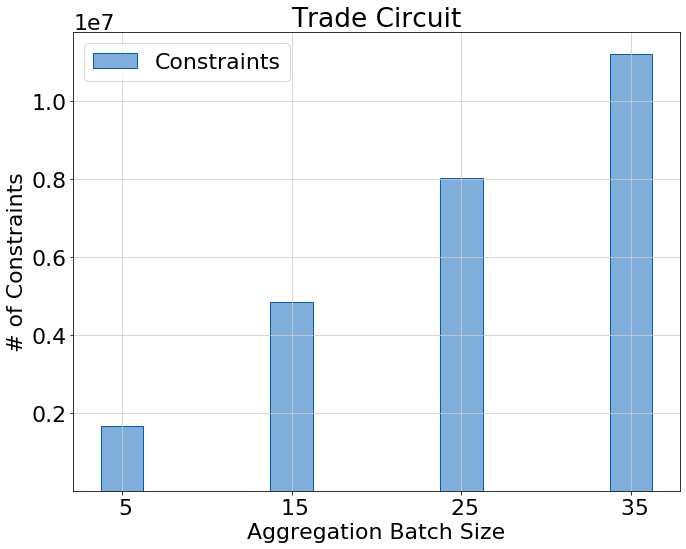
\includegraphics[width=5.9225cm]{diagrams/results_final_trade-constraints.png} }%
    \qquad
    \subfloat[]{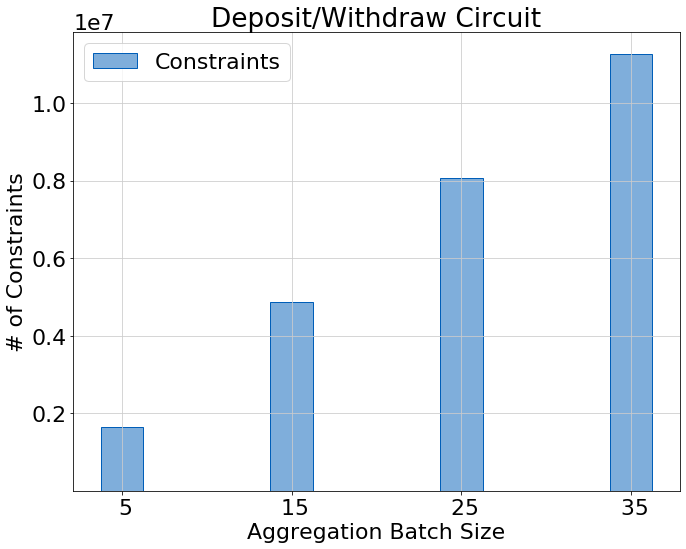
\includegraphics[width=5.9225cm]{diagrams/results_final_dep-constraints.png} }%
    \caption{Constraint count for the circuits in different batch sizes}%
    \label{fig:constraints}%
\end{figure}

\paragraph{subsubsection}{Origin of Constraints}
Both circuits can be broken down into three different main segments, that add a certain number of constraints. 1) We need to run the inclusion proof and update the merkle tree. 2) We check the signature and if the balance update follows the signed amounts. 3) We need to compute the data hash. For each of these operations, we get constraint numbers that are added per addition batch element. These numbers where measured by compiling the segments seperatly and checking the constraint count. Comparing these to the total constraint values, we realize that they are higher. This can be explained by the ZoKrates optimizer, which runs a number of optimizations during compilation. As we can see, these values are very similar in both circuits, which is why they have comparable performance.

\begin{table}[h]
    \begin{tabular}{lll}
    \toprule
                                  & Fixed Cost: & Variable Cost:     \\ \hline
    \multicolumn{3}{l}{\textbf{Trade Circuit:}}                      \\ \hline
    \midrule
    Merkle Tree                   & 1          & 179781              \\ \hline
    Verify sig and balance update & 1175       & 25675               \\ \hline
    Data hash                     & 182254     & 184806              \\ \hline
    \multicolumn{3}{l}{\textbf{Deposit/Withdraw Circuit:}}           \\ \hline
    \midrule
    Merkle Tree                   & 1          & 179781              \\ \hline
    Verify sig and balance update & 1          & 28154               \\ \hline
    Data hash                     & 55970      & 184806              \\ \hline
    \bottomrule
    \end{tabular}
\end{table}

\paragraph{subsubsection}{Hashing and Constraints}
The MiMC hashing algorithm was used for hashing the merkle tree, as it’s more efficient to use in zkSNARK circuits. The most common hashing operation used in the system is the pair hashing of the merkle tree. Every balance update requires 32 pair hashes in total, 16 for the merkle inclusion proof, and 16 for updating the merkle tree. We must also remember, that the pair elements need to be sorted according to their position (left, right), which doubles the constraints in a zkSNARK circuit. On the other hand, we also need to hash the balances in the zkSwap smart-contract for recreating the data hash. In Solidity the sha256 hashing algorithm is a lot cheaper than MiMC. Since we have to recreate the data hash for every batch we want to verify on-chain, the data hash is computed with the SHA256 hashing algorithm. 

\begin{table}[h]
    \begin{tabular}{lll}
    \toprule
    Hashing Op         & Constraints & Gas Usage \\  \hline
    \midrule
    MiMC pair          & 2642        & 94052    \\  \hline
    MiMC pair sorted   & 5285        & 94052    \\  \hline
    SHA256 pair        & 56227       & 1722     \\  \hline
    SHA256 pair sorted & 112453      & 1722     \\  \hline
    \bottomrule
    \end{tabular}
\end{table}

\paragraph{subsubsection}{Constraints Processed per Second}
As last metric we want to take a look at, is constraints processed per second in the witness computation and proof generation step. We can calculate these values by dividing the exectution time by the number of constraints. At the time of writing, these steps are not parallelizable and only run on one CPU core. The Loopring protocol claims to have parallelized the libsnark library, which we will look at in S. XX. For this reason we are introducing this metric, as we can compare the outcomes and the potential speed up of parrallelizing. On top of that, this metric can also be helpful to test the performance of the circuits on a CPU with higher clock speed.

\begin{table}[]
    \begin{tabular}{lll}
    \toprule
    batch\_size & Witness constraints / sec & Proof constraints / sec \\
    \midrule
    5           & 27604                     & 9685                    \\
    15          & 29615                     & 8417                    \\
    25          & 29088                     & 9612                    \\
    35          & 27797                     & 8382                    \\
    \midrule
    Average     & 28526                     & 9024                    \\
    \bottomrule 
    \end{tabular}
\end{table}